\begin{myQA}{编译到 \filename{eu1lmr.fd} 时很慢怎么办?}
	据说,只有在 Windows 系统上用 \hologo{XeTeX} 编译时才会出现这种情况。
	\hologo{XeTeX} 会调用系统字体,安装新字体后,需要刷新字体缓存,
	以使 \hologo{XeTeX} 识别新安装的字体。
	可以使用 \verb|fc-cache -f| 命令来重建字体缓存。
	
	关于 \verb|fc-cache| 更多用法,可以输入 \verb|fc-cache --help| 来查看。
	
	在 Mac 上,由于不使用 \filename{fontconfig} 机制,
	因此不会出现该问题。
	
	\myRef{\citet{TSE2015eu1lmr}}
\end{myQA}

\begin{myQA}{cmbright 字体为什么有锯齿?}
	因为
\end{myQA}

\begin{myQA}{如何使用好看的数学字体?}
	\TeX 和 \LaTeX 的默认字体是高老爷子制作的 Computer Modern,
	如图~\ref{Fig:cm_1} 所示。
	%	\begin{equation*}
	%		\int\sin^2 x \,\mathrm{d} x
	%		=\frac{1}{2}x - \frac{1}{4} \sin 2x + C
	%	\end{equation*}
	
	\begin{figure}[h]
		\centering
		\framebox{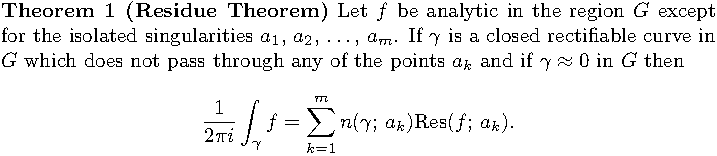
\includegraphics{Examples/cm_1}}
		\caption{Computer Modern 字体示例}
		\label{Fig:cm_1}
	\end{figure}
	
	好看是好看,但是多了也觉得乏味。下面推荐几个字体宏包,给诸位换换口味。
	
	首先是 CM Bright(图~\ref{Fig:cmbright}),这是一个能与
	Computer Modern 相配的无衬线字体,包含在 \pkg{cmbright} 宏包中。
	使用方法是在导言区加上 \verb|\usepackage{cmbright}|。
	
	CM Birght 有一个缺点:少了积分、求和等巨算符。默认采用
	Computer Modern 显示,处女座自是不会满意。不过稍费工夫,
	也有办法改用其他字体(Iwona 之类)。
	%TODO:20160827 需要引用其他问题
	
	\begin{figure}[h]
		\centering
		\framebox{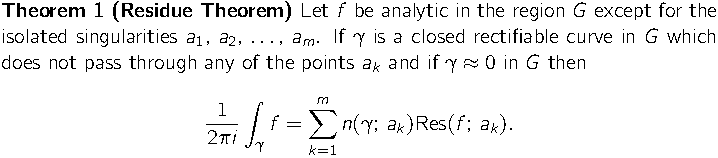
\includegraphics{Examples/cmbright}}
		\caption{CM Bright 字体示例}
		\label{Fig:cmbright}
	\end{figure}
	
	接下来是熟知的 Times 系列。
	
	\begin{figure}[h]
		\centering
		\framebox{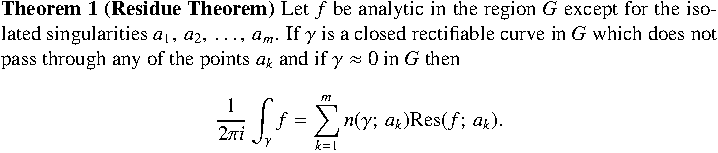
\includegraphics{Examples/txfonts}}
		\caption{Times 字体示例}
		\label{Fig:txfonts}
	\end{figure}
	
	\begin{figure}[h]
		\centering
		\framebox{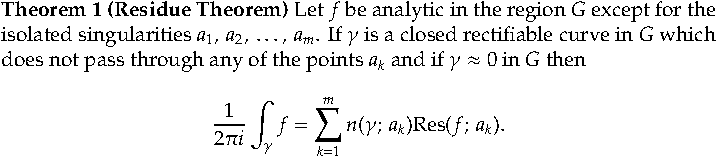
\includegraphics{Examples/pxfonts}}
		\caption{Palatino 字体示例}
		\label{Fig:pxfonts}
	\end{figure}
\end{myQA}

\begin{myQA}{如何使用更好看的数学字体?}
\end{myQA}